% This is "sig-alternate.tex" V1.9 April 2009
% This file should be compiled with V2.4 of "sig-alternate.cls" April 2009
%
% This example file demonstrates the use of the 'sig-alternate.cls'
% V2.4 LaTeX2e document class file. It is for those submitting
% articles to ACM Conference Proceedings WHO DO NOT WISH TO
% STRICTLY ADHERE TO THE SIGS (PUBS-BOARD-ENDORSED) STYLE.
% The 'sig-alternate.cls' file will produce a similar-looking,
% albeit, 'tighter' paper resulting in, invariably, fewer pages.
%
% ----------------------------------------------------------------------------------------------------------------
% This .tex file (and associated .cls V2.4) produces:
%       1) The Permission Statement
%       2) The Conference (location) Info information
%       3) The Copyright Line with ACM data
%       4) NO page numbers
%
% as against the acm_proc_article-sp.cls file which
% DOES NOT produce 1) thru' 3) above.
%
% Using 'sig-alternate.cls' you have control, however, from within
% the source .tex file, over both the CopyrightYear
% (defaulted to 200X) and the ACM Copyright Data
% (defaulted to X-XXXXX-XX-X/XX/XX).
% e.g.
% \CopyrightYear{2007} will cause 2007 to appear in the copyright line.
% \crdata{0-12345-67-8/90/12} will cause 0-12345-67-8/90/12 to appear in the copyright line.
%
% ---------------------------------------------------------------------------------------------------------------
% This .tex source is an example which *does* use
% the .bib file (from which the .bbl file % is produced).
% REMEMBER HOWEVER: After having produced the .bbl file,
% and prior to final submission, you *NEED* to 'insert'
% your .bbl file into your source .tex file so as to provide
% ONE 'self-contained' source file.
%
% ================= IF YOU HAVE QUESTIONS =======================
% Questions regarding the SIGS styles, SIGS policies and
% procedures, Conferences etc. should be sent to
% Adrienne Griscti (griscti@acm.org)
%
% Technical questions _only_ to
% Gerald Murray (murray@hq.acm.org)
% ===============================================================
%
% For tracking purposes - this is V1.9 - April 2009

\documentclass{sig-alternate}

\begin{document}

\title{Course Planning Model}

%\titlenote{(Produces the permission block, and
%copyright information). For use with
%SIG-ALTERNATE.CLS. Supported by ACM.}}
%\subtitle{[Extended Abstract]
%\titlenote{A full version of this paper is available as
%\textit{Author's Guide to Preparing ACM SIG Proceedings Using
%\LaTeX$2_\epsilon$\ and BibTeX} at
%\texttt{www.acm.org/eaddress.htm}}}
%
% You need the command \numberofauthors to handle the 'placement
% and alignment' of the authors beneath the title.
%
% For aesthetic reasons, we recommend 'three authors at a time'
% i.e. three 'name/affiliation blocks' be placed beneath the title.
%
% NOTE: You are NOT restricted in how many 'rows' of
% "name/affiliations" may appear. We just ask that you restrict
% the number of 'columns' to three.
%
% Because of the available 'opening page real-estate'
% we ask you to refrain from putting more than six authors
% (two rows with three columns) beneath the article title.
% More than six makes the first-page appear very cluttered indeed.
%
% Use the \alignauthor commands to handle the names
% and affiliations for an 'aesthetic maximum' of six authors.
% Add names, affiliations, addresses for
% the seventh etc. author(s) as the argument for the
% \additionalauthors command.
% These 'additional authors' will be output/set for you
% without further effort on your part as the last section in
% the body of your article BEFORE References or any Appendices.

\numberofauthors{8} %  in this sample file, there are a *total*
% of EIGHT authors. SIX appear on the 'first-page' (for formatting
% reasons) and the remaining two appear in the \additionalauthors section.
%
\author{
\alignauthor
Luyi Wang\\
       \affaddr{Lane of CSEE Department}\\
       \affaddr{West Virginia University}\\
       \affaddr{Morgantown, West Virginia}\\
       \email{lwang10@mix.wvu.edu}
}
\date{30 July 1999}
% Just remember to make sure that the TOTAL number of authors
% is the number that will appear on the first page PLUS the
% number that will appear in the \additionalauthors section.

\maketitle
\begin{abstract}

This paper proposed an intelligent course planning agent model which is based on {\em Actory} model.{\em Actory} model is a generic agent model which can be applied into diverse fields by enriching with specific domain knowledge. It utilizes BDI \cite{Rao91modelingrational} model as its archetype.  Simulations generated from it are aimed to illustrate real world scenarios where randomness and bias coexist due to undetermined events happening and environment changeableness within specific domain context.  With accumulatively learning and modeling improvement, ideally an actory model would be able to provide people suggestions on principles which can be derived to a comfortable life pattern.  This paper explains a course planning model which is used to assist academic institutes in planning undergraduate level courses.  This model consists of two sub agents. One is life event producer who takes in charge of generating life changing events which mimics the real life happening. The other is Course actor.  It plays an important role in this model where it simulate a real course provider which dispatches exams and gives out grades.  This work is motivated by the problem of automatically arranging course according to their dependency chain and meanwhile relieve the pressure from heavy course work caused by non-systemetic course planning.   
\end{abstract}

% A category with the (minimum) three required fields
%A category including the fourth, optional field follows...
\category{D.2.8}{Software Engineering}{Metrics}[complexity measures, performance measures]

\terms{Agent Modelling}

\keywords{Actory mode, course planning}

\section{Introduction}
Course planning is always a challenge issue for academic institutions.  A well defined course planning system would promote the educational quality by arranging course through prerequisite chain. Meanwhile it would relieve student's pressure in confronting with heavy workload and help them build up a systemic knowledge system.  With more and more research carrying on this area, some obvious demands are also brought in. First is the matrix structure of course prerequisite chain.  There is no obviously cut-off line to separate courses according to their easiness levels.  Some high-level theoretical courses are usually build upon rudimental courses which are provided in certain years. A certain number of courses focus more on practice and experiment which asks for  knowledge from both theoretical and implementation.  Second is how to seek a trade off between the flexibility of timeline and credit hour requirement.  Usually a college level degree requires student get at least 130 credit hours in 4 years.  With these motivation, an course planning system built upon existing academic requirement is required,accompany with adaptive to the dynamic prerequisite chain and flexibilities on course credit hour. \\

This paper proposed an approach to building such a agent technologies based one of BDI agent framework, Actory,  with the domain specific knowledge for course planning.   It utilizes the notion of generic programming and first-order agent language to fulfill above requirements. In section 2,  it introduces some notions of generic programming used in this system and also explains the framework of actory. Section 3 focus on describing the logic view of course planning model and details its implementation. Section 4 briefly shows up some experimental result.  The end section, Section 5, concludes current research status and point out the future work. \\

\section{Actory Model and its generic notions}
Agent oriented programming puts much more effect on adapting with dynamic environment changing by acquiring new coming in user requirements\cite{bresciani04}.   The whole system evolution progress  are also divided into separate phrases by specific requirements  according to agent oriented programming notions.  An empirical agent architecture, BDI\cite{rao1991mra} , are widely applied on current agent based system.  It brings in a mature mentalistic notions which helps the developer and users to interpret the logic underneath the agent based system.\\

\subsection{Actory Model}
 \textbf{ Actory Model}, a under developing agent model, also utilize BDI notions to reveal the methodology on domain-specific agent programming level.  This Model consists of three components: Factory, Machine and Transitions and system actor \cite{Levesque94golog:a}. 
 The system actor, called App, is introduced to control the whole work flow in the system. The component Factory plays an important roles in the system as a coordinator who gather all kind of resources and allocate them according to dynamic requirement from machines. Machine itself is regarded as an interactive agent who can dynamically load transitions who takes charge of fulfills task and communicates between machines.  Fig.1 is the basic Architecture of Actory Model. \\

\begin{figure}[h]
\centering
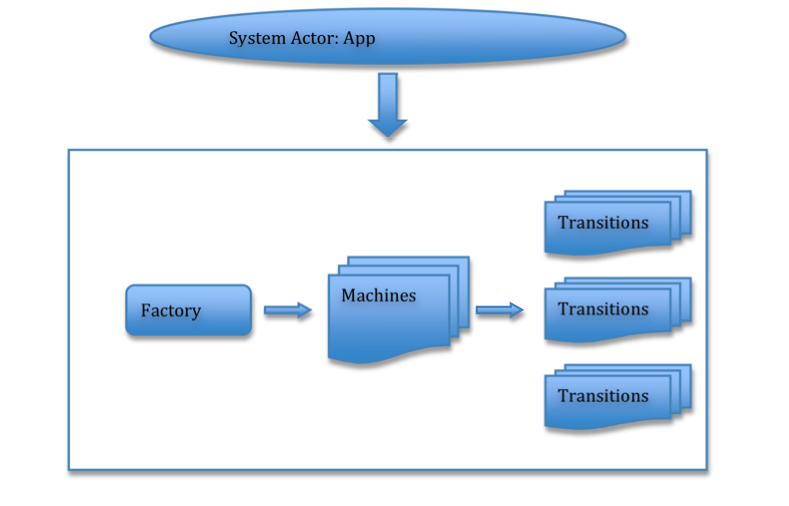
\includegraphics[width=90mm ]{actorymodel.png}
\caption{Actory Model Structure}
\end{figure}

Based on above architecture, we can see the logic underneath the system is quite obvious with one to many mapping, wherever one factory can contains more than one machines while machine can hold up at least one transitions.  To solve the resource conflicts and reach the concurrency requirement, a semaphore named "asynchronous" is introduced into "App" system actor.  Moreover, this structure provides a framework for enriching with domain specific knowledge without caring environments. Specific domain level programming can be derived from upper level as factory or machine as sub-agent. Meanwhile, tasks on specific domains are implemented as transitions which are gathered and submitted to the domain factory through domain machines. 
\subsection{Generic Notions}
As we discussed in the actory model, we can see several notions, such as factory, machines,etc, are essential in defining the BDI architecture for this model.  Before we proceed to give out the detail notions, we first examine the structure of this components.  The factory component contains one factor called {\em patience} which is controlled by the system actor app.  When the factory loses its temper, or the system actor app reach its limits, defined as {\em toomuchloops},  the system  is terminated.   To this point, we can regard the system's final belief as keep patience and keep running for fulfilling all tasks.  Correspondingly,  the machine component has several constraints on state checking, which is related to the transition component.  The transition component states the adaptation of environment by bringing in condition examine an switching.  The {\em guard} condition determines what the {\em next} state is, and  meanwhile {\em sideeffect} controls the system status changing, such as push hard to lose patience.   So here we can see the desire in actory is trying to keep the patience as many as possible and intention is to fulfill the task by switching to {\em normal state} instead of to {\em loop state }or {\em error state}.   So till here, we can use the Table 1. to illustrate the logic view underneath the system.
\begin{table}[h]
\centering
\caption{BDI notions in Actory Model}
\begin{tabular}{|c|c|c|}\hline
Component Name & BDI Notions & Factor Name \\
\hline
Factory & Belief & Patience\\
\hline
Machine & Desire & Start \\
\hline
Transition & Intention & Next,Guard, SideEffect \\
\hline
\end{tabular}
\end{table}

\section{Course Planning Domain Specific Model}
As we narrated before, course planning is an essential part in academic education.  Based on actory model, we can simulate a virtual college environment in which students take courses and enjoy their college life by participate event like football game.  This is also the feature of actory model, domain specific programming.  \\

\subsection{CP Model Structure}
To enrich actory with domain specific feature, we have to derived component from actory model and brings in sub-system actory which acts as a coordinator in resource allocation and communication. Here we derived two classes from {\em Machine} component as {\em Course} and {\em Student}.    To generate tasks for these two new components ,we invented two sub-system actors as {\em CourseEvent} and {\em LifeEvent}, respectively creating events for course and student life.  Fig 2. Show the Course Planning Model Structure after introducing more components.\\
\begin{figure}[!h]
\centering
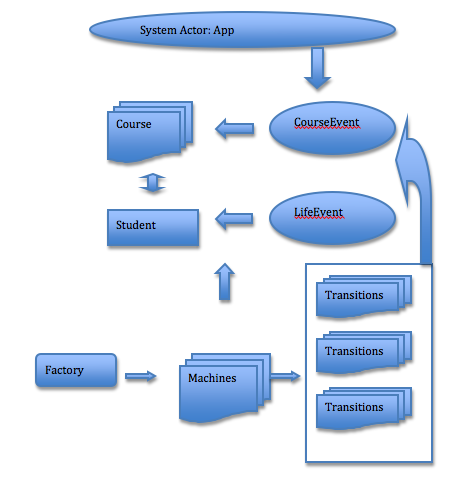
\includegraphics[height=90mm ]{courseplanmodel.png}
\caption{Course Planning Model Structure}
\end{figure}

\subsection{CP BDI Notions}
This two sub-system actor still use the patience to control its work flow and termination state.  So it stills use actory BDI mentalism.  For the student component, we bring in one factor called {\em happiness} to extend its belief.  So from a student perspective, he/she would like to live with happiness and without losing their temper.  To reach this point, they need to seek a balance between life and academic workload.   But this structure doesn't affect the original BDI mentalism established in the actory model. Table 2 gives out the extended BDI architecture in course planning model.\\
\begin{table*}
\centering
\caption{BDI notions in Course Planning Model}
\begin{tabular}{|l|l|l|l|}\hline
Component Name & Derived Componet & BDI Notions & Factor Name \\
\hline
App & Object & System Actor & Patience\\
\hline
CourseEvent, LifeEvent & App & Sub-system Actor & Patience\\
\hline
Factory & Factory  & Belief & Patience\\
\hline
Student, Course & Machine & Desire & Patience, Happiness \\
\hline
Transition& Transition & Intention & Next,Guard, SideEffect \\
\hline

\end{tabular}
\end{table*}

\subsection{CP Work Mechanism}
In this course plan model, student actively choose courses which is disordered.  Correspondingly, subsystem actor, {\em Lifeevent}, would dynamically generate life events while another {\em courseevent} is generating course events for the course the student taken.  The factor {\em happiness} defined in the student component determines the number of events the student can hold.  When some positive activities, such as {\em win lottery}, take place, the happiness value would be raised up.  Oppositely, the negative activity would reduce the happiness value, such as getting bad grades for exam.  When the events generated, the system actor patience is losing till it enter its termination states where we defined as patience value to 0. Current design doesn't allow the patience value can increase which would lead to an endless state. Also to prevent this happen, a factor called index is introduced in subsystem factor to control the maximum event number which is set as 50.\\

Also as we stressed before, the Course Plan Model should conquer challenges of course matrix prerequisite chain.  In this course plan model,  each course has its corresponding prerequisite chain which can be looked up. An already taken course would relieve patience of sub-system actor,{\em course event}, to deduct the number of events which is generated automatically.  This is fair in real life situation.  Also this mechanism would solve the matrix problem by indexing courses, which is currently not implemented. \\ 

\section{Experiment Results}
Usually running time efficiency is always an important factor in evaluating computation model. However since the dynamic events are generated with time delay, to evaluate this course model by its running time is not executable.  To reach this deal, the number of events generated in certain amount of time becomes to be essential.   Currently all the experiment results is just calculated by this scale.  Before we show the experimental, we should first define the initial value used in this model as table 3 shows.
\begin{table}[h]
\centering
\caption{Initial value in CP Model }
\begin{tabular}{|c|c|c|}\hline
Factor name & Component Name & Initial Value \\
\hline
patience & SubS,System Factors & 100\\
\hline
happiness & Student &100\\
\hline
index & subsystem Factory &0\\
\hline
\end{tabular}
\end{table}


{\secit Experimental  result is lacked due to knowledge constrains.}


\section{Conclude and Future work}
In this paper, we proposed a new course planning model established upon actory model.  This course plan model is trying to simulate the students life by mimic real life event.  It implemented under BDI mentalism and fulfill the requirement of agent programming. However 
this course plan model is still under developing with more features need to be added, such as courses indexing and others.   Also the current concurrent model is hardly relies on delay which would cost too much computing time on waiting. Some semaphores need to be introduced to solve this problem.  In the future, more work would be done on this model.  

\bibliographystyle{IEEEtran}
\bibliography{sig-alternate}
\end{document}
